\section{如何将 {\LaTeX} 文档转换为 Word}

如果你决定使用 {\LaTeX} 进行论文撰写,但是你的导师希望你提供 Word 版本的论文进行方便的批注等,你可以使用下面的方法来将你的 {\LaTeX} 论文转换为 Word 格式的文档。需要注意的是,这种方式的转换并不能完整的将 {\LaTeX} 论文的全部格式进行转换,仅能保证正文部分内容的不丢失,其余包括“论文封面”、“表格”等等部分的内容,在转换的过程中都可能丢失。这些部分需要你后期手动进行添加。

\subsection{安装 Pandoc 命令行工具}

Pandoc 是一个支持几乎所有 Markup 格式文档的“通用文档转换器”,是一个命令行工具,支持所有常用操作系统。我们可以借助 pandoc 进行格式转换。

Pandoc 详细的安装说明请见官方文档:\href{https://pandoc.org/installing.html}{Installing pandoc}.

简单来说:

\begin{itemize}
  \item 在 Windows 上:
  \begin{itemize}
    \item 你可以使用 scoop 包管理工具安装 pandoc(为了方便设置命令行工具的环境变量,推荐使用 scoop 进行安装):
    \begin{minted}[frame=single]{bash}
    scoop install pandoc
    \end{minted}
    \textbf{关联阅读:}\href{https://sspai.com/post/52496}{“一行代码”搞定软件安装卸载,用 Scoop 管理你的 Windows 软件}
    \item 当然你也可以直接在 \href{https://github.com/jgm/pandoc/releases/latest}{Pandoc 的 GitHub Release 页面} 下载 Windows MSI 安装文件手动安装
  \end{itemize}
  \item 在 macOS 上你可以使用 Homebrew 包管理工具安装 pandoc:
  \begin{minted}[frame=single]{bash}
  brew install pandoc
  \end{minted}
  \item 在 Linux 上你可以使用你所用发行版的包管理工具安装 pandoc,比如:
  \begin{minted}[frame=single]{bash}
  sudo apt install pandoc
  \end{minted}
\end{itemize}

之后,在终端中输入:
\begin{minted}[frame=single]{bash}
  pandoc --version
\end{minted}

如果出现类似下面的输出,说明你的 pandoc 安装成功。

\begin{figure}[H]
  \centering
  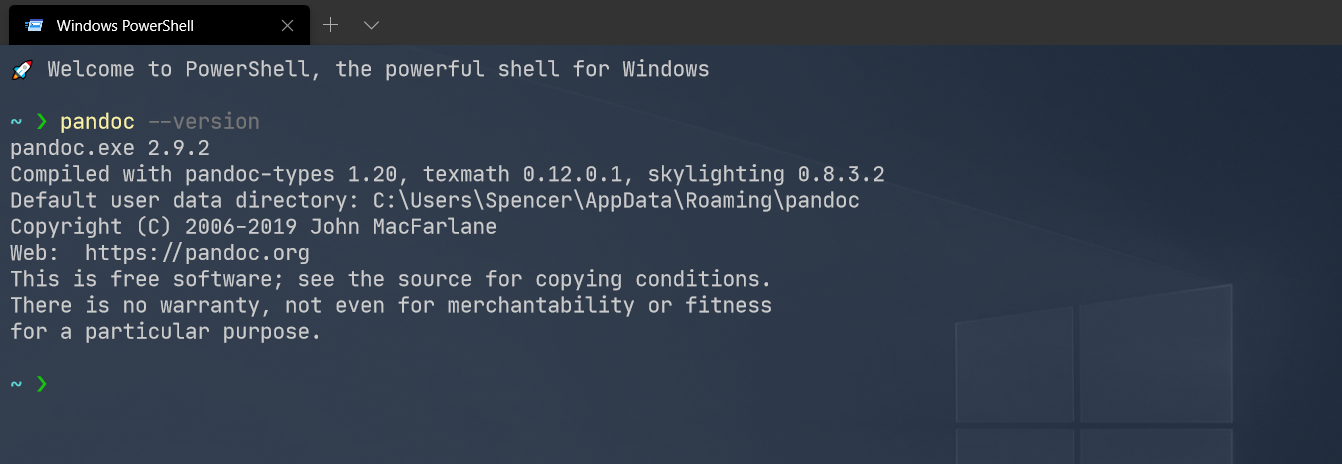
\includegraphics[width=\textwidth]{images/pandoc_test.png}
  \caption{测试 pandoc 安装成功}
  \label{pandoc_test}
\end{figure}

\subsection{完善 Word 格式的模板文件}

为了保证导出的 Word 文档格式和学校提供的模板大体一致,我们需要确认 Word 版本的模板\textbf{已经准确定义了各级标题、正文等部分的格式。}

\begin{figure}[H]
  \center
  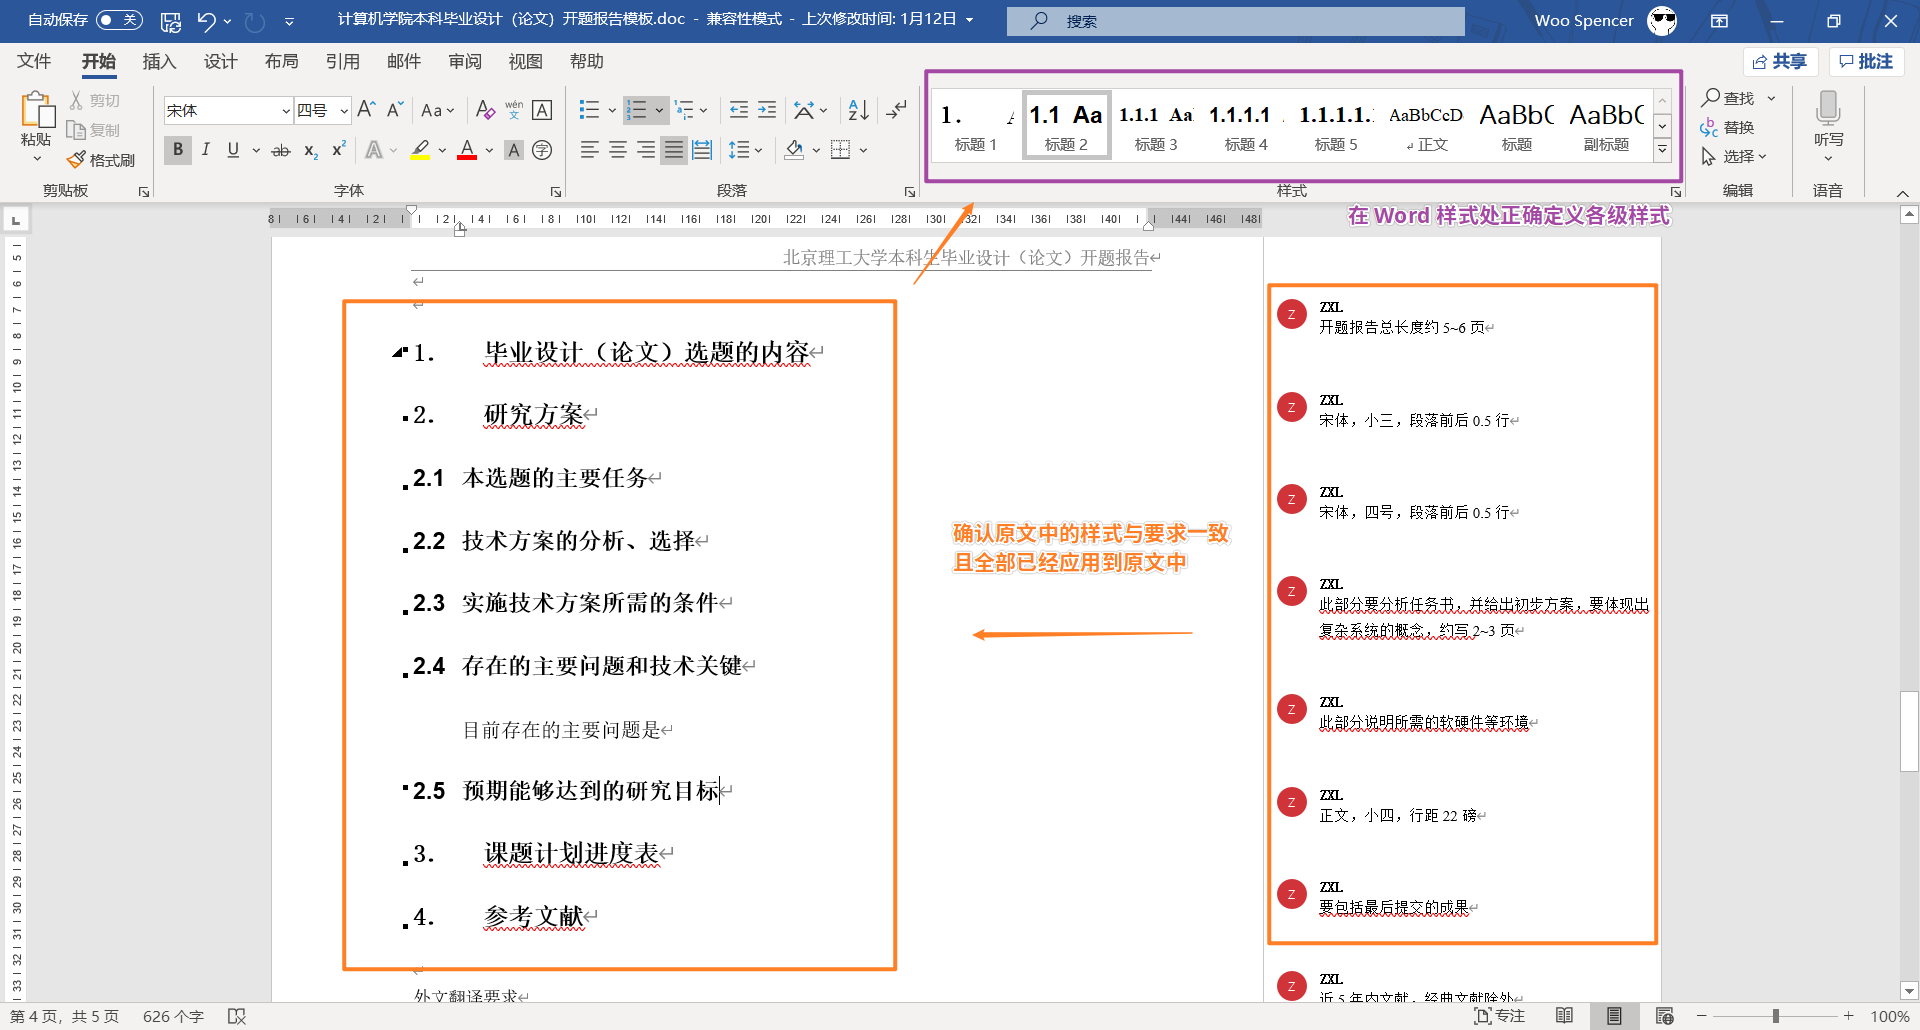
\includegraphics[width=\textwidth]{images/latex_pandoc_word.png}
  \caption{确认 Word 版本的模板准确生成}
  \label{latex_pandoc_word}
\end{figure}

之后,我们需要将这一文件(\texttt{doc} 或 \texttt{docx})保存,\textbf{留作 pandoc 的格式参考。}

\subsection{进行格式转换}

最后,我们进行格式的转换。

\subsubsection{朴素格式转换}

如果你只希望将文本内容导出为 Word,不在意格式或其他内容的正确性,你可以直接使用下面的命令进行最普通的文本转换:

\begin{minted}[frame=single]{bash}
  pandoc {LaTeX 文档文件} -o {输出 Word 文档}
\end{minted}

比如:

\begin{minted}[frame=single]{bash}
  pandoc main.tex -o main.docx
\end{minted}

没有特别指明模板 Word 文档格式与参考文献文档的情况下,pandoc 仅会处理你 {\LaTeX} 文档中的文字内容,按照标题、正文的格式整理进入 Word。

\subsubsection{含有目标模板 Word 文档的格式转换}

如果你希望按照模板 Word 文档的规定格式进行转换,那么你可以直接使用下面的命令进行格式转换:

\begin{minted}[frame=single,linenos,breaklines]{bash}
  pandoc {LaTeX 文档文件} --reference-doc={参考模板 Word 文档} -o {输出 Word 文档}
\end{minted}

比如,我们的 {\LaTeX} 文档文件名称为 \texttt{main.tex},参考模板 Word 文档名称为 \texttt{template.docx},希望输出名为 \texttt{main.docx} 的 Word 文档,我们即可如下组织 pandoc 转换命令:

\begin{minted}[frame=single]{bash}
  pandoc main.tex --reference-doc=template.docx -o main.docx
\end{minted}

\subsubsection{含有参考文献文档的格式转换}

如果你的 LaTeX 文档中包含有参考文献的引用,那么你需要特别明确参考文献 \hologo{BibTeX} 文件,将文件以 \texttt{--bibliography=\{参考文献文件\}} 的参数告知 pandoc,从而让 pandoc 正确处理你的参考文献。比如:

\begin{minted}[frame=single,linenos,breaklines]{bash}
  pandoc main.tex --bibliography=refs.bib --reference-doc=template.docx -o main.docx
\end{minted}

特别强调:pandoc 格式转换功能有限,无法处理 {\LaTeX} 多级嵌套表格(在本模板的“开题报告”与“毕业论文”中都有使用多级嵌套表格,直接调用 pandoc 默认情况下会报错。需要删掉 {\LaTeX} 文档中的表格,并后期手动录入 Word 之中),也无法保证格式与 {\LaTeX} 原文档 \textbf{完全一致},都需要我们后期手动进行调整。
